\documentclass{article}
\usepackage{cmap}
\usepackage{multicol}
\usepackage[top=3cm,bottom=3cm,left=3cm,right=3cm]{geometry}
\usepackage{hyperref}
\usepackage{graphicx}
\usepackage{caption}
\usepackage{capt-of}
\newenvironment{Figure}
  {\par\medskip\noindent\minipage{\linewidth}}
  {\endminipage\par\medskip}

\title{Forrest Fire Simulation model}
\author{Tom Peerdeman - 10266185 \& Ren\'e Aparicio Saez - 10214054}

\begin{document}

\maketitle

\begin{abstract}
\textbf{Le Abstract.}
\end{abstract}

\begin{multicols}{2}

\subsection*{Introduction}
Forest fires can spread in various ways and can be effected by a lot of environmental variables. The way a fire spreads between flammable objects for example can make a huge difference in the way a forest fire moves. Fire can also be affected by environmental variables, like water, the weather or wind. Manmade objects and people can interfere with the fire as well. Fire fighters can try to extinguish fire to keep the fire from spreading. Paths and roads, like water cannot be set on fire. It is however possible for fire to cross roads and some streams of water if the conditions are right. All these variables have to be taken into account when simulating a forest fire.\\\\
Forest fire simulations can be created by using cellular automata. Most cellular automata models consist of certain rules to change a cell’s state. While it is possible to use rules to simulate a forest fire, probabilities are used in order to simulate the environmental effects on the forest fire.

\subsection*{Defining the neighborhoods}
\subsubsection*{Different grids}
In order to ensure that the simulation is applicable in many situations, three different types of grids were used to simulate forest fires. These grids are: the Cartesian grid, the hexagonal grid and the triangular grid. Each grid has a different spread of fire.\\\\
For the Cartesian grid a straightforward method is used. By using a Moore neighborhood the eight squares around the current square can be directly influenced. The neighborhood is shown in figure \ref{fig:cartesianstd}.\\\\
The hexagonal grid could be positioned in two different ways. Either with flat sides of the hexagon along the y-axis, or with the flat sides along the x-axis. Both types of hexagons will do, by changing your perspective on the simulation, it is possible to simulate the other type of hexagon. For the experiments and simulations the type with sides along the x-axis is chosen. As shown by \cite{HernandezEncinas20071213}, hexagonal grids show a slight difference in mathematics when they are either odd or even (in this case along the x-axis). The neighborhood is shown in figure \ref{fig:hexstd}.  \\\\
Just like the hexagonal grid, the triangular grid can be placed in two different ways. Either along the y-axis or the x-axis. Again, the latter is chosen, to keep consistency for both grids. Whereas the fire spread of the Cartesian and the hexagonal grids are the same, no matter the location, the spread of the triangular grid differs per position. The triangle can either point up or down, switching along each axis. The neighborhoods for the triangles are shown in figure \ref{fig:triangle1std} and figure \ref{fig:triangle2std}.
\begin{Figure}
 \centering
 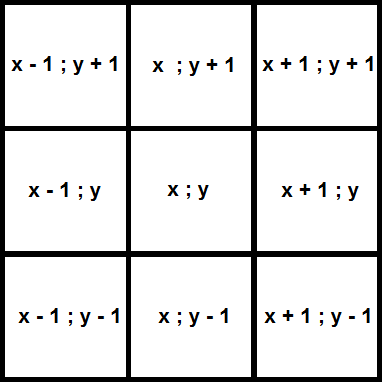
\includegraphics[width=0.79\textwidth]{imgs/cartesian.png}
 \captionof{figure}{Cartesian grid neighborhood}
\label{fig:cartesianstd}
\end{Figure}
\begin{Figure}
 \centering
 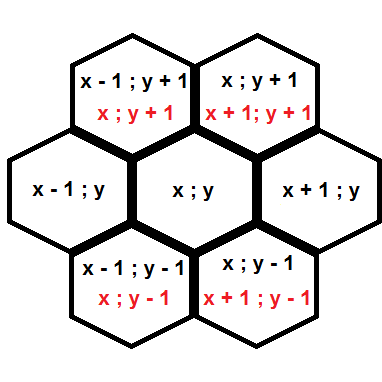
\includegraphics[width=0.79\textwidth]{imgs/hexagonal.png}
 \captionof{figure}{Hexagonal grid neighborhood}
\label{fig:hexstd}
\end{Figure}
\begin{Figure}
 \centering
 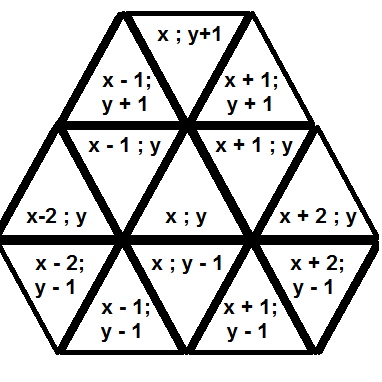
\includegraphics[width=0.79\textwidth]{imgs/triangle1.png}
 \captionof{figure}{Triangle 1 grid neighborhood}
\label{fig:triangle1std}
\end{Figure}
\begin{Figure}
 \centering
 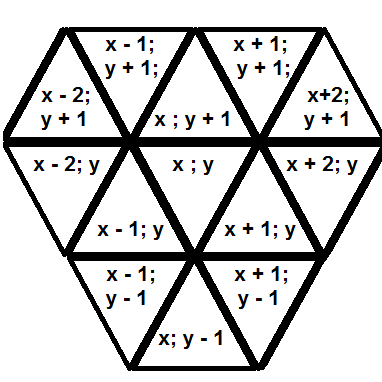
\includegraphics[width=0.79\textwidth]{imgs/triangle2.png}
 \captionof{figure}{Triangle 2 grid neighborhood}
\label{fig:triangle2std}
\end{Figure}

\subsubsection*{Spread probabilities}
Each grid can be initialized with certain probabilities for their neighborhoods. These probabilities represent the probability of fire to spread to the specific cell. By using probabilities, instead of a guaranteed fire spread, different types of situations can be used when simulating the fire. By changing the probabilities in certain ways, different types of weather, wind and terrain can be simulated. For example, when the weather is rainy, the probabilities can be set lower, while when it’s hot the probabilities can be set higher. The same goes for wind, if the wind blows in a certain direction, the probabilities for that direction can be set higher than the other directions.\\\\
In order to increase the environmental factor even more, it is also possible to influence cell's outside the neighborhood. In this way, extreme hot weather or high wind speeds can be simulated even better. When this feature is used, a new probability is created for fire to spread to a cell with a distance of two cell's from the current cell. This probability is calculated by dividing the interpolated probabilities of the cell's in the neighborhood in the direction of the cell outside the neighborhood by a given number. This way, the probability for fire to spread is always equal or lower to the probabilities of the cell's its probability was interpolated from.\\
The areas that could catch fire if the spread of distance two is enabled is shown in the following figures. Note that the area of the triangles is a bit odd. The area that would have been able to get on fire if all the surrounding cell's were used, was too big in comparison to the other grids. Because of that the area for the triangles has been reduced. The extended neighborhoods are shown in gray in figures \ref{fig:extcartesianstd},  \ref{fig:exthexstd},  \ref{fig:exttriangle1std} and  \ref{fig:exttriangle2std}.\\\\
Besides the increased environmental factor, the extended neighborhood also has as advantage that it can simulate fire moving across water and paths. This is a very useful feature. If this wasn't the case, fire could never spread even when facing a small river or path. Combined with this feature, the spread can simulate more 'actual world like' forest fires.
\begin{Figure}
 \centering
 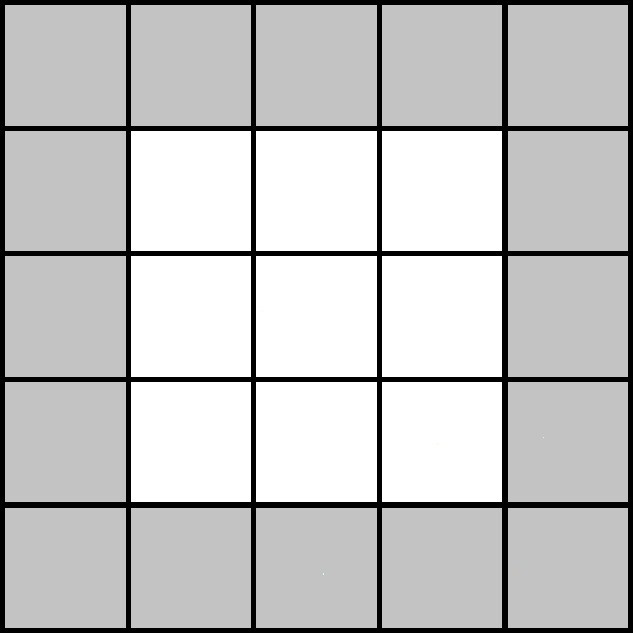
\includegraphics[width=0.79\textwidth]{imgs/extendedcartesian.png}
 \captionof{figure}{Extended Cartesian grid neighborhood}
\label{fig:extcartesianstd}
\end{Figure}
\begin{Figure}
 \centering
 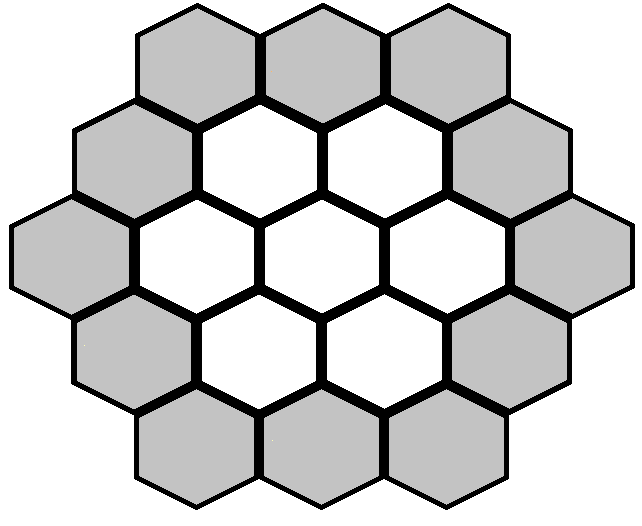
\includegraphics[width=0.79\textwidth]{imgs/extendedhexagonal.png}
 \captionof{figure}{Extended Hexagonal grid neighborhood}
\label{fig:exthexstd}
\end{Figure}
\begin{Figure}
 \centering
 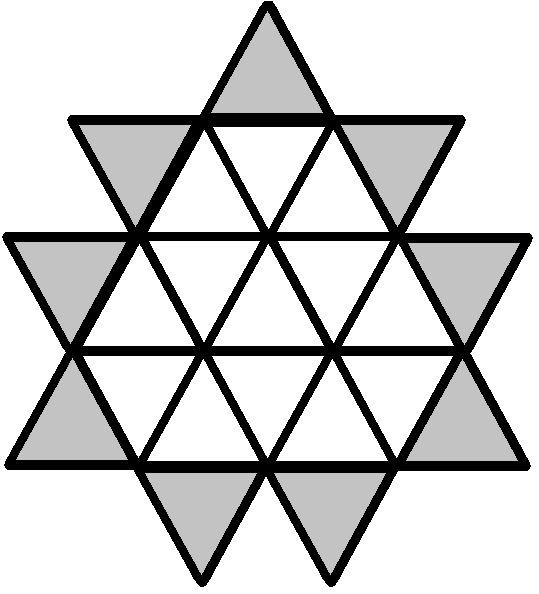
\includegraphics[width=0.79\textwidth]{imgs/extendedtriangle1.png}
 \captionof{figure}{Extended Triangle1 grid neighborhood}
\label{fig:exttriangle1std}
\end{Figure}
\begin{Figure}
 \centering
 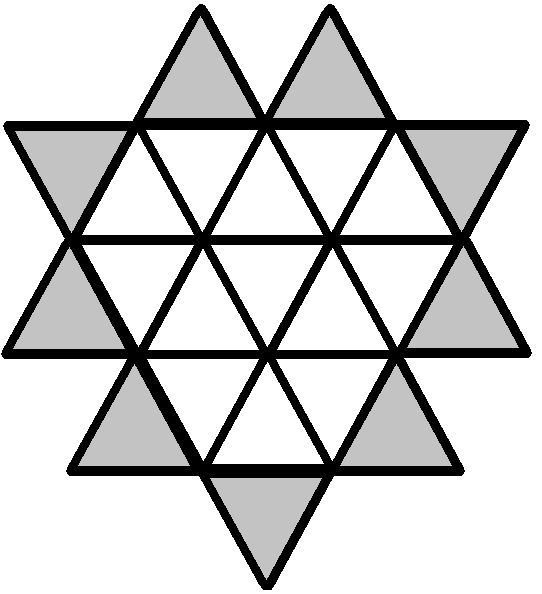
\includegraphics[width=0.79\textwidth]{imgs/extendedtriangle2.png}
 \captionof{figure}{Extended Triangle2 grid neighborhood}
\label{fig:exttriangle2std}
\end{Figure}

\subsection*{Core}
\subsection*{Experiments}
\subsection*{Results}
\subsection*{Interpretation}

\subsection*{Discussion \& Conclusion}

\subsection*{References}
\end{multicols}
\newpage
\bibliographystyle{plain}
\bibliography{RDC4}
\end{document}
